\documentclass[12pt,letterpaper]{article}
\usepackage[utf8]{inputenc}
\usepackage[margin=1in]{geometry}
\usepackage{graphicx}
\usepackage{titling}
\usepackage{amsmath}
\usepackage{amsfonts}
\usepackage{amssymb}
\renewcommand{\theenumiv}{\arabic{enumiv}}
\setlength{\droptitle}{-5em}
\author{Maurice Diesendruck}
\title{MCMC HW 3}
\usepackage{Sweave}
\begin{document}
\Sconcordance{concordance:hw3.2.tex:hw3.2.Rnw:%
1 12 1 1 0 81 1}

\maketitle


\paragraph{(a)}

\begin{equation}
Pr(y_i=1|X_i) = \Phi(X_i'\beta).
                     \end{equation}
                     \begin{equation}
                     y_i = I(z_i > 0)
                     \end{equation}
                     \begin{equation}
                     z_i \sim\ N(X_i'\beta, 1)
\end{equation}

Show that $(1) \equiv (2) \text{ and } (3)$: \\
First, "$\Leftarrow$" $(2) \text{ and } (3) \text{ imply }$
  
  \begin{displaymath}
y_i = \left\{
  \begin{array}{lr}
  1  :& z_i > 0 \text{, or when } z_i=X_i'\beta + \epsilon_i >0 \Rightarrow \epsilon_i > -X_i'\beta\\
  0  :& \text{otherwise}
  \end{array}
  \right.
  \end{displaymath}
  
  Where $z_i = X_i'\beta+\epsilon_i \text{, } \epsilon \sim\ N(0,1)$.\\
  
  So, $P(y_i=1|X_i) = P(z_i>0) = P(\epsilon_i>-X_i'\beta) = P(\epsilon_i < X_i'\beta) = \Phi(X_i'\beta) \equiv$ (1).\\

The inequality in the penultimate step is allowed to switch signs by the symmetry of the Normal distribution.\\

\paragraph{(b)}

Find conditional posterior $P(z_i|\beta, y)$ and $P(\beta|z,y)$, using prior on $\beta$, $P(\beta)=1$.\\

The conditional posterior of $z_i$ is identical to (3), except that the given value of $y_i$ informs the value of $z_i$, by definition.

\begin{displaymath}
z_i|\beta,y \sim\ \left\{
  \begin{array}{lr}
  N(X_i'\beta, 1), \text{ left truncated at $0$, if } y_i=1\\
    N(X_i'\beta, 1), \text{ right truncated at $0$, if } y_i=0
  \end{array}
  \right.
  \end{displaymath}
  
  In summary, if $y_i=1$ then the distribution is the right side of the normal distribution centered at $X_i'\beta$, whereas if $y_i=0$ then the distribution is the left side.\\

The conditional posterior of $\beta$, given a flat, uninformative prior, is simply the standard least squares result on the Normal $z$:

\begin{equation}
\beta|z,y \sim\ N(\hat{\beta_z}, 1 \cdot (X'X)^{-1})
\end{equation}
\begin{equation}
\text{Where } \hat{\beta_z} = (X'X)^{-1}X'z
\end{equation}



\paragraph{(c)}

Gibbs sampler proposition:\\
Initialize value for $\beta$ as MLE, and call it $\beta_0$. Then set $\beta_0=\beta_k$.
\begin{enumerate}
\item Sample $z_k$ from $P(z_k|\beta_k,y)$.
\item Sample $\beta_{k+1}$ from $P(\beta_{k+1}|z_k,y)$.
\item Repeat until convergence and good mixing.
\end{enumerate}

After discarding values from the beginning of the chain (the burn in period), the resulting values of $\beta$ and $z$ will be an estimate of the exact joint posterior distribution $P(\beta, z | y)$.

\paragraph{(d)}

Show the histogram of simulated $\beta$ values as an estimate of $p(\beta_j|y)$.

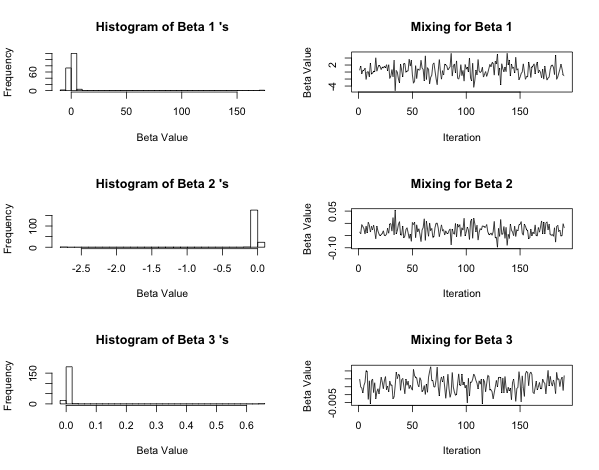
\includegraphics[width=150mm,scale=1.5]{hw32pic.png}

\end{document}
